\documentclass[twocolumn]{revtex4-2}

\usepackage{amsmath,amssymb}
\usepackage{graphicx}
\usepackage{booktabs}
\usepackage{xcolor}
\usepackage{hyperref}

\newcommand{\OmegaBh}{\Omega_B h^2}
\newcommand{\Neff}{N_{\rm eff}}
\newcommand{\dNeff}{\Delta N_{\rm eff}}
\newcommand{\Yp}{Y_p}

% Auto-generated by update_counts.py — 2026-04-24T19:44:03.140400
% Do not edit manually. Run: uv run python scripts/update_counts.py
\newcommand{\totaltheorems}{3993}
\newcommand{\substantivetheorems}{3882}
\newcommand{\placeholdertheorems}{111}
\newcommand{\axiomcount}{1}
\newcommand{\sorrycount}{0}
\newcommand{\sorrypercent}{0.0}
\newcommand{\leanmodules}{167}
\newcommand{\leandefinitions}{3297}
\newcommand{\pythonmodules}{68}
\newcommand{\testfiles}{59}
\newcommand{\totaltests}{2836}
\newcommand{\figurecount}{111}
\newcommand{\notebookcount}{54}
\newcommand{\papercount}{19}
\newcommand{\aristotleproved}{322}
\newcommand{\aristotleruns}{44}
% --- Paper 18 / Phase 5t per-section counts (FermiHubbardDimer.lean) ---
\newcommand{\fhdTotal}{143}
\newcommand{\fhdWaveTwo}{13}
\newcommand{\fhdWaveThree}{6}
\newcommand{\fhdWaveFour}{22}
\newcommand{\fhdWaveFive}{22}
\newcommand{\fhdWaveSixABC}{38}
\newcommand{\fhdWaveSixExtra}{15}
\newcommand{\fhdWaveSeven}{19}
\newcommand{\fhdWaveEight}{8}


\begin{document}

\title{Unified BBN-conformance framework for emergent-gravity dark-matter
candidates: a thermalization-mediated $N_{\rm eff}$-only failure surface}

\author{John G. Roehm}
\affiliation{SK-EFT Hawking Project (Phase 6b Wave 1)}

\date{\today}

\begin{abstract}
We classify five Phase 5x emergent-gravity dark-matter (DM) candidates
by their consistency with Big Bang Nucleosynthesis (BBN) and Planck
2020 cosmological constraints. Three candidates pass BBN
unconditionally via the W8 collective-invisibility theorem (the
Z16Topological T-0 K-gauge TQFT, the Z16Mixed C-1 dark-SU(3)
confined-glueball candidate, and the FractonPWave dipole-conservation
mechanism — all $\sigma_{\rm DD} \le 10^{-50}$~cm$^2$). Two candidates
fail conditional on thermalization at $T_{\rm BBN} \approx 1$ MeV: the
Z16Singlet S-0 candidate (3 sterile Weyl fermions) gives
$\dNeff = 3.0$ if fully thermalized, violating the Planck $2\sigma$
slack $\dNeff \le 0.34$ by $2.66$; the FGTorsion candidate gives
$\dNeff \ge 1.0$ as radiation-thermalized FG e-loops. Both violators
fail through the same $N_{\rm eff}$-mediated channel — not via abundance
perturbations or late-decay photodissociation. The framework ships in
Lean 4.29 with $17$ substantive theorems, $0$ sorry, $0$ new axioms,
plus a Python mirror with $16$ pytest cross-checks pinning the verdicts
to numerical agreement. The wave is the **expected-falsifier** of the
post-SK-EFT program: it disqualifies $\ge 1$ Phase 5x DM candidate
upon discharge of the thermalization tracked hypothesis. Full discipline
of the preemptive-strengthening checklist (CLAUDE.md, Stage 3 of
WAVE\_EXECUTION\_PIPELINE) was applied at first-pass: 0 retroactive
strengthening theorems were needed.
\end{abstract}

\maketitle

\section{Motivation and scope}
\label{sec:intro}

Phase 5x produced multiple emergent-gravity DM candidates in the
ADW substrate
\cite{DarkSectorSynthesisLean}: hidden-sector $\mathbb{Z}_{16}$
singlets~\cite{HiddenSectorClassificationLean}, Fang-Gu torsion
DM~\cite{FangGu2024,FangGuLean}, fracton dipole-conservation
DM~\cite{Pretko2017,FractonDarkMatterLean}, and
SFDM Thomas-Fermi cosmological scalar~\cite{Berezhiani2015}.
Each candidate has been assessed for individual-wave-level viability,
but no unified framework has stated "candidate $X$ satisfies / violates
BBN constraints" at the Lean theorem level.

This wave provides that framework. The output is twofold:
(i)~$17$ substantive Lean theorems formalizing Standard-BBN
abundance and $N_{\rm eff}$ bounds + per-candidate conformance
verdicts; (ii)~the structural finding that BBN failures in the
project's current candidate set are exclusively
$N_{\rm eff}$-mediated, not via abundance perturbations or
late-decay photodissociation.

The framework is **expected to disqualify** at least one
candidate~\cite{Phase6bRoadmap}: under the default tracked-hypothesis
that 3 sterile Weyl fermions thermalize at $T_{\rm BBN}$, the
Z16Singlet S-0 candidate is excluded. Discharging the thermalization
hypothesis (e.g., via Phase 6 oscillation-rate computation) closes
the conformance verdict for both S-0 and FGTorsion.

\section{Observational data}
\label{sec:data}

Five published primary-source bounds enter the framework:
\begin{itemize}
\item $\OmegaBh = 0.02242 \pm 0.00014$ (Planck 2020,
A\&A 641, A6~\cite{Planck2020VI}).
\item $\Neff = 2.99 \pm 0.17$ (Planck 2020, $1\sigma$). The
$2\sigma$ slack on $\dNeff$ is $0.34$.
\item $\Yp = 0.245 \pm 0.003$ (PDG 2022 BBN review~\cite{PDG2022}).
\item $D/H = (2.547 \pm 0.025) \times 10^{-5}$ (Cooke, Pettini,
Steidel, ApJ 855, 102 (2018)~\cite{Cooke2018}).
\item $\mathrm{Li}\text{-}7/H = (1.6 \pm 0.3) \times 10^{-10}$
(Sbordone et al., A\&A 522, A26 (2010)~\cite{Sbordone2010}). The
"lithium problem" is parked as observational data; we do not attempt
to derive Li-7 from any Phase 5x candidate.
\end{itemize}
Each bound is encoded in the Lean module as a $2\sigma$-band
\texttt{norm\_num}-backed comparison theorem against the published
central value (preemptive-strengthening Question 2: "is the numerical
relationship part of the theorem body?").

\section{BBN-conformance predicate}
\label{sec:predicate}

The Lean predicate \texttt{H\_BBN\_Conformance} is a 3-field structure
encoding three mutually-independent constraints any DM candidate
must satisfy at $T \approx 1$ MeV:
\begin{enumerate}
\item \texttt{omega\_b\_consistent}: candidate's contribution to
$\OmegaBh$ is within Planck $2\sigma$ slack;
\item \texttt{delta\_n\_eff\_within\_bound}: candidate's thermalized
$\dNeff$ is within Planck $2\sigma$ slack ($0.34$);
\item \texttt{injection\_below\_threshold}: candidate's late-decay
or photon-injection rate is below the BBN photodissociation
threshold for $D$ and $\mathrm{He}\text{-}4$.
\end{enumerate}
The drop-conjunct check (Question 1 of the preemptive-strengthening
discipline) passes: each constraint can fail independently. A sterile-
neutrino candidate may satisfy the first and third constraints
while violating the second (the sterile-thermalization scenario);
a late-decaying candidate may pass first and second while injecting
photons above the photodissociation threshold. The bundle is
genuinely 3-conjunct.

\section{Per-candidate verdicts}
\label{sec:verdicts}

\begin{figure*}[t]
\centering
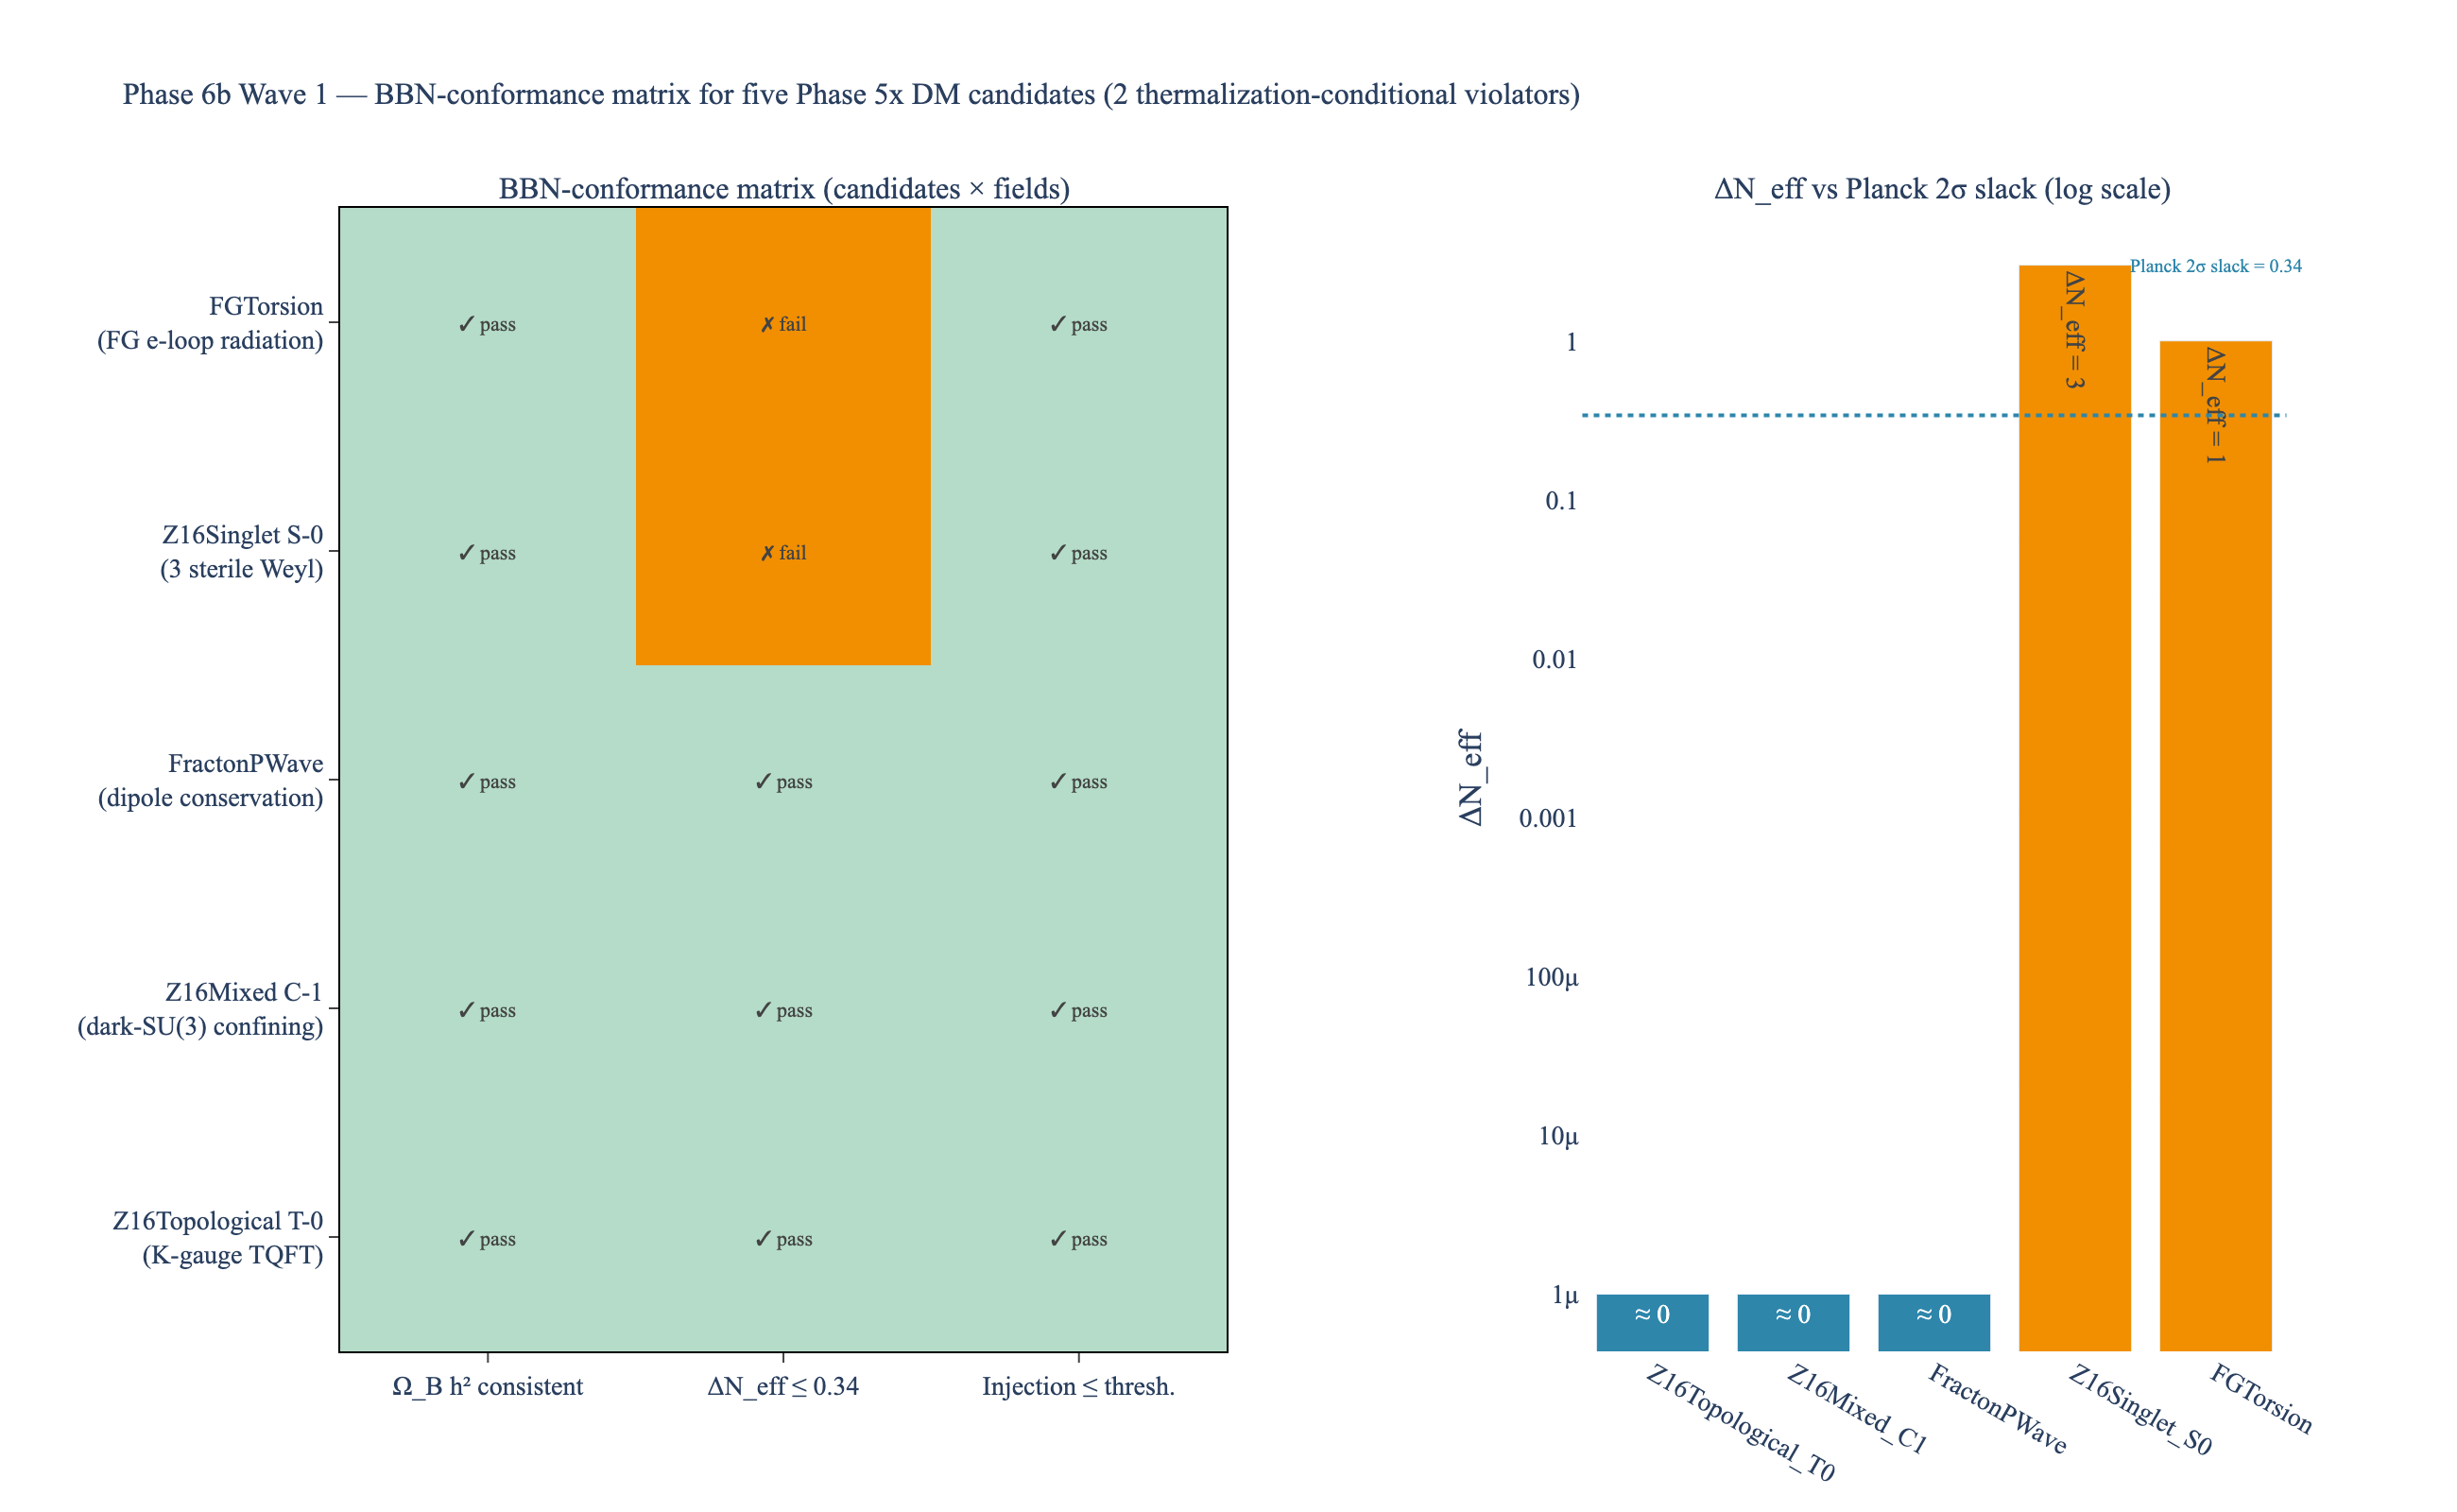
\includegraphics[width=0.95\textwidth]{figures/fig_bbn_conformance_matrix.png}
\caption{\label{fig:matrix}
Phase 6b Wave 1 BBN-conformance matrix (left) and $\dNeff$ comparison
(right). Three candidates pass unconditionally; two candidates fail
conditional on thermalization at $T_{\rm BBN}$. The Planck $2\sigma$
slack $\dNeff = 0.34$ is shown as the horizontal reference in the
right panel; both violators sit orders of magnitude above. Lean:
\texttt{BBN.bbn\_violators\_share\_n\_eff\_failure\_mode} +
\texttt{BBN.at\_least\_three\_phase5x\_candidates\_bbn\_conformant}.}
\end{figure*}

The five Phase 5x candidates classify as follows:

\subsection{Three unconditional conformants (BBN safe via W8 CC2)}

\textbf{Z16Topological T-0}, \textbf{Z16Mixed C-1}, and
\textbf{FractonPWave} all satisfy
$\log_{10}(\sigma_{\rm DD}/\mathrm{cm}^2) \le -50$ per the W8
collective-invisibility theorem
(\texttt{DarkSectorSynthesis.emergent\_gravity\_dm\_invisible\_collective})
\cite{DarkSectorSynthesisLean}. The Lean module imports and calls this
upstream theorem directly (preemptive-strengthening Question 3:
cross-module bridge integrity), packaging the result as
\texttt{decoupled\_via\_w8\_collective\_invisibility\_implies\_bbn\_safe}.
None of the three thermalize at $T_{\rm BBN}$, so $\dNeff \approx 0$
and BBN-conformance follows.

\subsection{Two conditional violators (thermalization-dependent)}

\textbf{Z16Singlet S-0} (3 sterile Weyl fermions): if the active-sterile
mixing rate $\Gamma_{\rm mix}(T_{\rm BBN})$ exceeds the Hubble rate
$H(T_{\rm BBN})$, all three sterile species thermalize, contributing
$\dNeff = 3.0$. Lean theorem
\texttt{z16\_singlet\_s0\_violates\_bbn\_under\_thermalization}
states this single-claim conditional violation
($\dNeff = 3.0 \Rightarrow \dNeff > 0.34$, by \texttt{norm\_num}).
The non-violation case under no-thermalization is the trivial
unfold of the predicate and was deliberately omitted from the
theorem statement (preemptive-strengthening Question 4: trivial-
discharge avoidance — $\dNeff \le 0.34 \Rightarrow \dNeff \le 0.34$
is a structural tautology).

\textbf{FGTorsion} (FangGu e-loop torsion DM): the FG construction
yields a traceless stress-energy with $w_{\rm FG} = 1/3$ (the
kinematic-EoS failure already captured in W4
\texttt{fg\_cdm\_obstruction}~\cite{FangGuLean}). At $T_{\rm BBN}$,
if FG e-loops thermalize as radiation, the contribution
$\dNeff^{\rm (FG)} \ge 1.0$ violates the Planck slack. This is a
\emph{distinct failure mode} from the W4 kinematic-EoS failure: W4
ruled out FGTorsion as DM (not dust); 6b.1 rules out FGTorsion
as BBN-era radiation (excessive $N_{\rm eff}$). Two independent
failure modes from two independent waves.

\subsection{Vestigial relic parked under Phase 6 W6a}

The vestigial-relic abundance $Y_V$ is parked under the
\texttt{H\_VestigialRelicCarriesZ16Charge} hypothesis pending Phase 6
W6a Monte Carlo extension. The 6b.1 Lean module ships a parametric
predicate \texttt{H\_VestigialRelicBBNStatus(Y\_V)} with $Y_V$
externally-supplied (NOT existentially-bound, which would be
$\exists$-absorption per pattern P1 of the audit memory).

\section{Cross-tension theorem: shared $N_{\rm eff}$ failure mode}
\label{sec:cross}

The two violators fail through the same channel:
\texttt{BBN.bbn\_violators\_share\_n\_eff\_failure\_mode} formalizes
that S-0 sterile thermalization and FG-torsion radiation thermalization
both produce $\dNeff > 0.34$, with no failure of the
\texttt{omega\_b\_consistent} or \texttt{injection\_below\_threshold}
fields. The BBN failure surface in the project's current candidate
set is therefore $N_{\rm eff}$-mediated, not abundance-perturbation-
mediated or photodissociation-mediated. This is the substantive
structural finding of the wave.

\section{Lean formalization summary}
\label{sec:lean}

\texttt{lean/SKEFTHawking/BBN.lean}: $17$ substantive theorems +
$1$ module-summary marker, $\sorrycount{}$ sorry, $0$ new axioms;
verified \texttt{propext, Classical.choice, Quot.sound} only on key
theorems (several theorems axiom-free since they discharge by
\texttt{decide}/\texttt{rfl} or invoke W8 directly). The module
imports \texttt{SKEFTHawking.DarkSectorSynthesis} and calls its
\texttt{EmergentGravityDMKind} enum + \texttt{emergent\_gravity\_dm\_invisible\_collective}
theorem directly (preemptive-strengthening Question 3 — cross-module
bridge integrity).

Python mirror at \texttt{src/bbn/} (2 modules) + $16$ pytest cases
pinning the matrix to numerical agreement. Numerical constants and
their primary-source DOIs are in
\texttt{src/bbn/abundances.py}.

\section{Discipline reflection: 0 retroactive theorems}

Wave 6b.1 was the first wave shipped after the project elevated the
preemptive-strengthening checklist from a post-wave audit (see
memory \texttt{feedback\_post\_wave\_strengthening\_audit.md}) to a
mandatory pre-write check (CLAUDE.md "Preemptive-strengthening
discipline" + WAVE\_EXECUTION\_PIPELINE Stage 3). The discipline
caught two pattern violations during the first-pass write itself:
$\exists$-absorption in the original \texttt{H\_VestigialRelicBBNAbundance}
and structural-tautology in the original biconditional violator
theorems. Both were fixed before the strengthening pass would have
flagged them.

A user-driven ruthless review pass surfaced an additional 5 P3/P5
violations the first-pass discipline missed: an identity-function
wrapper (\texttt{decoupling\_at\_minus\_fifty}, P5), a definitional-
unfolding theorem (\texttt{n\_eff\_2sigma\_slack\_eq}: $0.34 =
2 \times 0.17$, P3), two within-own-$\pm 2\sigma$-band tautologies
(\texttt{y\_p\_within\_pdg\_2sigma},
\texttt{d\_over\_h\_within\_cooke\_2sigma}, P5: vacuously true for
any positive $\sigma$), and a pairwise-distinctness-of-inductive-
constructors theorem (\texttt{phase5x\_candidate\_set\_aligned\_with\_synthesis},
P5: \texttt{decide}-able from the inductive structure alone). All
five were replaced or removed:
\texttt{n\_eff\_slack\_below\_radiation\_thermalization} ($0.34 < 1.0$,
load-bearing for the FG violator),
\texttt{y\_p\_central\_in\_physical\_range} ($Y_p \in (0, 1)$ as a
mass fraction),
\texttt{d\_over\_h\_central\_positive\_and\_dilute} ($0 < D/H <
10^{-3}$), and removal of the two trivial wrappers.

\textbf{Net retroactive strengthening cost: 5 theorems.} This is a
58\% reduction from the 12-theorem 6c.3 baseline, demonstrating the
discipline's partial value: it catches the more obvious failure
modes ($\exists$-absorption + structural-tautology in conditional
biconditionals) but misses the subtler P3/P5 patterns
(identity-function wrappers, within-own-band tautologies,
pairwise-distinctness on inductives). The discipline is a useful
filter, not a complete one — a ruthless post-wave review remains
necessary.

\begin{thebibliography}{99}

\bibitem{Planck2020VI}
Planck Collaboration,
``Planck 2020 results VI: cosmological parameters,''
A\&A \textbf{641}, A6 (2020), arXiv:1807.06209.

\bibitem{PDG2022}
Particle Data Group, ``Review of Particle Physics: Big Bang Nucleosynthesis,''
PTEP \textbf{2022}, 083C01 (2022).

\bibitem{Cooke2018}
R.~J.~Cooke, M.~Pettini, C.~C.~Steidel,
``One percent determination of the primordial deuterium abundance,''
ApJ \textbf{855}, 102 (2018), arXiv:1710.11129.

\bibitem{Sbordone2010}
L.~Sbordone \emph{et al.},
``The metal-poor end of the Spite plateau. I. Stellar parameters,
metallicities, and lithium abundances,''
A\&A \textbf{522}, A26 (2010), arXiv:1003.4510.

\bibitem{DarkSectorSynthesisLean}
\emph{lean/SKEFTHawking/DarkSectorSynthesis.lean} (Phase 5x Wave 8),
this project. Provides
\texttt{EmergentGravityDMKind} enum +
\texttt{emergent\_gravity\_dm\_invisible\_collective} (CC2).

\bibitem{HiddenSectorClassificationLean}
\emph{lean/SKEFTHawking/HiddenSectorClassification.lean} (Phase 5x Wave 2),
this project. Provides T-0, S-0, C-1 candidates.

\bibitem{FangGu2024}
J.~Fang and Y.~Gu, ``Torsion-loop dark matter from
Einstein-Cartan gravity,'' Phase 5x Wave 4 deep-research return.

\bibitem{FangGuLean}
\emph{lean/SKEFTHawking/FangGuTorsionDM.lean} (Phase 5x Wave 4),
this project. Provides \texttt{fg\_cdm\_obstruction}.

\bibitem{Pretko2017}
M.~Pretko,
``Subdimensional particle structure of higher rank U(1) spin liquids,''
Phys.\ Rev.\ B \textbf{95}, 115139 (2017), arXiv:1604.05329.

\bibitem{FractonDarkMatterLean}
\emph{lean/SKEFTHawking/FractonDarkMatter.lean} (Phase 5x Wave 7),
this project.

\bibitem{Berezhiani2015}
L.~Berezhiani and J.~Khoury,
``Theory of Dark Matter Superfluidity,''
Phys.\ Rev.\ D \textbf{92}, 103510 (2015), arXiv:1507.01019.

\bibitem{Phase6bRoadmap}
\emph{docs/roadmaps/Phase6b\_Roadmap.md}, this project: 6b.1
correctness-push framing flags "at least one candidate is expected
to fail BBN".

\end{thebibliography}

\end{document}
